\documentclass[a5paper,11pt]{extarticle}

\def\labauthors{Сарафанов Ф.Г., Платонова М.В.}
\def\labgroup{440}
\def\labnumber{2}
\def\labstartdate{12 марта}
\def\labtheme{Исследование принципов\\[-0.2em] статического управления \\[0.2em]
электронным потоком в триоде}
\def\shortlabtheme{Вакуумный триод}

%!TEX root = ../vdiode.tex
\usepackage{cmap}
\usepackage[T2A]{fontenc}
\usepackage[utf8x]{inputenc}
\usepackage[english, russian]{babel}

\usepackage{misccorr} % в заголовках появляется точка, но при ссылке на них ее нет
\usepackage{amssymb,amsfonts,amsmath,amsthm}  
\usepackage{indentfirst}
\usepackage[usenames,dvipsnames]{color} 
\usepackage[unicode,hidelinks]{hyperref}
% \hypersetup{%
%     pdfborder = {0 0 0}
% }

\usepackage{makecell,multirow} 
\usepackage{ulem}
\usepackage{graphicx,wrapfig}
\graphicspath{{img/}}
\usepackage{geometry}
\geometry{left=1.5cm,right=1.5cm,top=2cm,bottom=2cm,bindingoffset=0cm,headheight=15pt}
\usepackage{fancyhdr} 
\linespread{1.05} 
\frenchspacing 
\renewcommand{\labelenumii}{\theenumii)} 
\newcommand{\mean}[1]{\langle#1\rangle}
% \usepackage{caption}
%%%%%%%%%%%%%%%%%%%%%%%%%%%%%%%%%%%%%%%%%%%%%%%%%%%%%%%%%%%%%%%%%%%%%%%%%%%%%%%
%%%%%%%%%%%%%%%%%%%%%%%%%%%%%%%%%%%%%%%%%%%%%%%%%%%%%%%%%%%%%%%%%%%%%%%%%%%%%%%



%%%%%%%%%%%%%%%%%%%%%%%%%%%%%%%%%%%%%%%%%%%%%%%%%%%%%%%%%%%%%%%%%%%%%%%%%%%%%%%
	%применим колонтитул к стилю страницы
\pagestyle{fancy} 
	%очистим "шапку" страницы
\fancyhead{} 
	%слева сверху на четных и справа на нечетных
\fancyhead[L]{\labauthors} 
	%справа сверху на четных и слева на нечетных
\fancyhead[R]{\shortlabtheme} 
	%очистим "подвал" страницы
\fancyfoot{} 
	% номер страницы в нижнем колинтуле в центре
\fancyfoot[C]{\thepage} 
\renewcommand{\phi}{\varphi}
%%%%%%%%%%%%%%%%%%%%%%%%%%%%%%%%%%%%%%%%%%%%%%%%%%%%%%%%%%%%%%%%%%%%%%%%%%%%%%%

\usepackage{float}
\usepackage[mode=buildnew]{standalone}
\usepackage{tikz} 
% \usepackage{subcaption}
\usepackage{csvsimple}
\usetikzlibrary{scopes}
\usetikzlibrary{%
     decorations.pathreplacing,%
     decorations.pathmorphing,%
    patterns,%
    calc,%
    scopes,%
    arrows,%
    % arrows.spaced,%
}
\makeatletter
\newif\if@gather@prefix 
\preto\place@tag@gather{% 
  \if@gather@prefix\iftagsleft@ 
    \kern-\gdisplaywidth@ 
    \rlap{\gather@prefix}% 
    \kern\gdisplaywidth@ 
  \fi\fi 
} 
\appto\place@tag@gather{% 
  \if@gather@prefix\iftagsleft@\else 
    \kern-\displaywidth 
    \rlap{\gather@prefix}% 
    \kern\displaywidth 
  \fi\fi 
  \global\@gather@prefixfalse 
} 
\preto\place@tag{% 
  \if@gather@prefix\iftagsleft@ 
    \kern-\gdisplaywidth@ 
    \rlap{\gather@prefix}% 
    \kern\displaywidth@ 
  \fi\fi 
} 
\appto\place@tag{% 
  \if@gather@prefix\iftagsleft@\else 
    \kern-\displaywidth 
    \rlap{\gather@prefix}% 
    \kern\displaywidth 
  \fi\fi 
  \global\@gather@prefixfalse 
} 
\newcommand*{\beforetext}[1]{% 
  \ifmeasuring@\else
  \gdef\gather@prefix{#1}% 
  \global\@gather@prefixtrue 
  \fi
} 
\makeatother

\usepackage{booktabs}
\usepackage{pgfplots, pgfplotstable}

\usepackage[outline]{contour}
\usepackage{tocloft}
\renewcommand{\cftsecleader}{\cftdotfill{\cftdotsep}} % for parts
% \renewcommand{\cftchapleader}{\cftdotfill{\cftdotsep}} % for chapters
\usepackage{pgfplots,pgfplotstable,booktabs,colortbl}
\pgfplotsset{compat=newest}
\usepackage{physics}
\usepackage{mathtools}
\mathtoolsset{showonlyrefs=true}
\newcommand\Smat{\hat { \mathbf { S } }}

\newcommand*\dotvec[1][1,1]{\crossproducttemp#1\relax}
\def\crossproducttemp#1,#2\relax{{\qty[\vec{#1}\times\vec{#2}\,]}}

\newcommand*\prodvec[1][1,1]{\crossproducttempa#1\relax}
\def\crossproducttempa#1,#2\relax{{\qty[{#1}\times{#2}\,]}}

% \def\E{\mathscr{E}_H}
\def\Rdim{\,\frac{\text{м}^3}{\text{А} \cdot \text{с}}}

\renewcommand{\vec}{\mathbf} % for parts
\begin{document}
%!TEX root = ../diode.tex
\begin{titlepage}
\begin{center}
% \vspace{-3em}
{\small\textsc{Нижегородский государственный университет имени Н.\,И. Лобачевского}}
\vskip 2pt \hrule \vskip 3pt
{\small\textsc{Радиофизический факультет}}

\vfill


{{\large Отчет по лабораторной работе №\labnumber}\vskip 12pt {\LARGE \bfseries \labtheme}}

	
\vspace{2cm}
{\large Работу выполнили студенты \\[-0.25em] \labgroup\  группы радиофизического факультата \\[0.5em] {\Large \bfseries \labauthors}}

% \vspace{0.5cm}
% {e-mail: sfg180@yandex.ru}

% \vspace{2cm}

\end{center}

\vfill
	
% \begin{flushright}
% 	{Выполнили студенты 430 группы\\ \labauthor}%\vskip 12pt Принял:\\ Менсов С.\,Н.}
% \end{flushright}
	
% \vfill
	
\begin{center}
	{Нижний Новгород, \labstartdate\ -- \today}
\end{center}

\end{titlepage}

\tableofcontents
\newpage



\addcontentsline{toc}{section}{Введение}
\section*{Введение}
\vspace{-0.5em}
В настоящей работе изучаются принципы управления электронным потоком в триоде. В качестве активной среды выступает поток свободных электронов, движущихся в вакууме.Для преобразования кинетической энергии электронов в энергию ЭМП в электронном пучке должны быть периодические сгустки. В работе будет использоваться статический способ формирования электронных сгустков.
Триод может являться как усилителем тока, так и усилителем напряжения.
Триод характеризуется тремя величинами, которые будут измерены в работе: внутреннее сопротивление(отношение бесконечно малого приращения анодного напряжения к приращению анодного тока при постоянном напряжении на сетке), крутизна (отношение бесконечно малых приращений анодного тока и напряжения на сетке при постоянном напряжении на аноде), статический коэффициент усиления по напряжению (отношение бесконечно малого приращения напряжения на аноде к приращению напряжения на сетке при постоянном анодном токе).

\vspace{-0.5em}
 % Как показано в \cite[стр. ы]{met}

\paragraph{Установка.} Работа производится на установке, позволяющей собрать различные
схемы включения лампы триода. На установке задается анодное
напряжение с помощью потенциометра в пределах от 0 до 220 В,
напряжение с управляющей сетки снимается с помощью делителя
напряжения и также регулируется потенциометром.
Дя повышения точности измерения характеристик триода используется
метод переменной составляющей,для чего переменное напряжение
малой амплитуды (50-100мВ) подается на сетку лампы.
Снятие анодных и анодно-сеточных характеристик производится
одновременно с измерением параметров лампы 

\section{Эксперимент}
\subsection{Измерение анодно-сеточной характеристики триода} % (fold)
\begin{figure}[H]
	\centering
	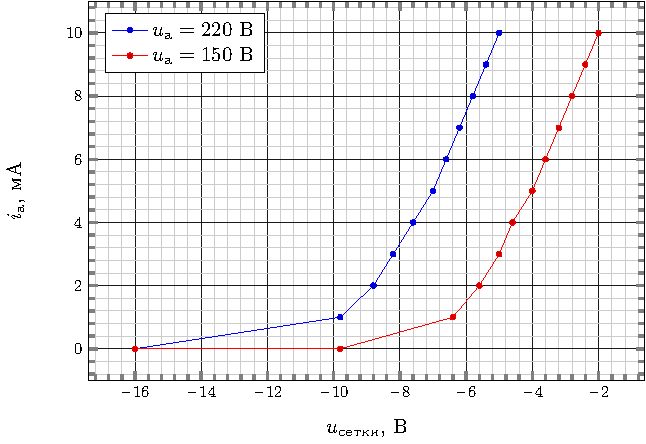
\includegraphics[]{fig/ia_from_uc.pdf}
	\vspace{-1em}
	\caption{Анодно-сеточная характеристика}
	\label{fig:1}
\end{figure}

В этом задании была снята анодно-сеточная характеристика при двух значениях анодного напряжения. Из графика видно, что чем больше напряжение на аноде, тем круче идет А-С характеристика. Это очевидно, так как чем больше напряжение на аноде, тем больше электроны ускоряются и тем больше у них вероятность попасть на анод.
По анодно-сеточной характеристике крутизна рассчитывается слеюущим образом: 
\begin{gather}
	S_a=\frac{U_out}{U_in}\frac{1}{R_a}
\end{gather}
\begin{figure}[H]
	\centering
	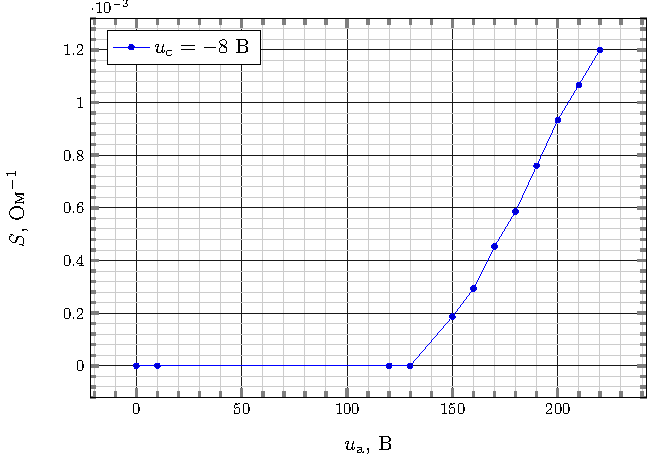
\includegraphics[]{fig/s_from_ua.pdf}
	\vspace{-1em}
	\caption{Зависимость крутизны от напряжения на аноде}
	\label{fig:1}
\end{figure}

При увеличении напряжения на сетке или аноде, крутизна также увеличивается.
\subsection{Измерение анодной характеристики триода}
В этом задании была снята зависимость анодного тока от напряжения на аноде для двух различных напряжениях на сетке:
\begin{figure}[H]
	\centering
	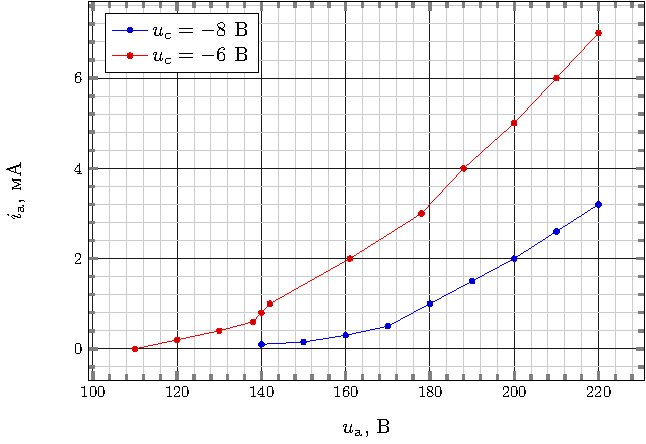
\includegraphics[]{fig/ia_from_ua.pdf}
	\vspace{-1em}
	\caption{Анодная характеристика триода}
	\label{fig:1}
\end{figure}

Из графика видно, что при увеличении по модулю сеточного напряжения, анодная характеристика поднимается вверх. Это означает, что большее количество электронов достигает анода при большем значении напряжения на сетке.
По анодной характеристике внутреннее сопротивление рассчитывается следующим образом:
\begin{gather}
	R = \frac{U_{in}}{U_{out}} R_a
\end{gather}
\begin{figure}[H]
	\centering
	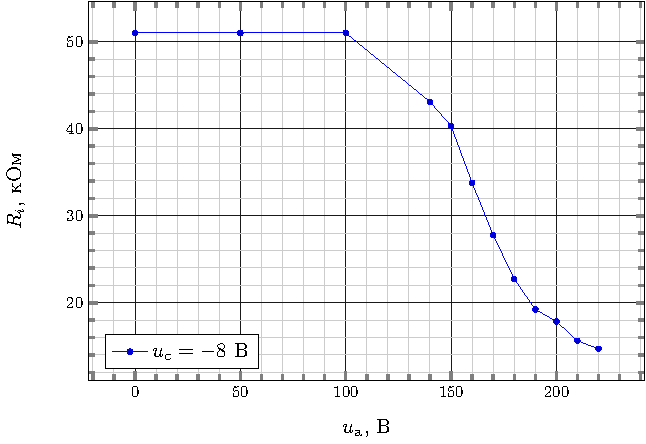
\includegraphics[]{fig/r_from_ua.pdf}
	\vspace{-1em}
	\caption{Зависимость внутреннего сопротивления от анодного напряжения}
	\label{fig:1}
\end{figure}

При увеличении анодного напряжения и постоянном сеточном напряжении внутреннее сопротивление уменьшается. 
\begin{figure}[H]
	\centering
	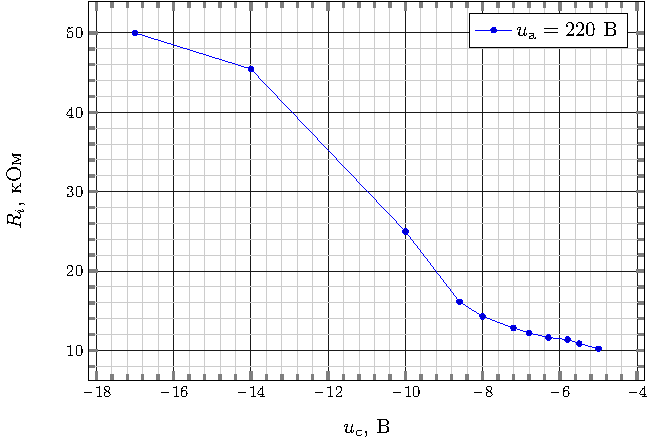
\includegraphics[]{fig/r_from_uc.pdf}
	\vspace{-1em}
	\caption{Зависимость внутреннего сопротивления от сеточного напряжения}
	\label{fig:1}
\end{figure}

При уменьшении модуля сеточного напряжения и постоянном анодном напряжении внутреннее сопротивление уменьшается.
% \newpage
\subsection{Измерение статического коэффициента усиления по напряжению} 
Для этого необходимо воспользоваться внутренним уравнением триода:
\begin{gather}
	\mu = S R_i
\end{gather}

\begin{figure}[H]
	\centering
	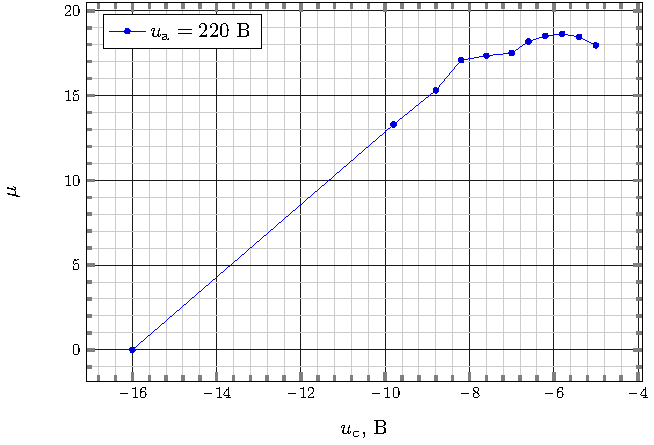
\includegraphics[]{fig/mu_from_uc.pdf}
	\vspace{-1em}
	\caption{Зависимость $\mu$ от напряжения на сетке}
	\label{fig:1}
\end{figure}
C уменьшением по модулю напряжения на сетке статический коэффициент усиления по напряжению увеличивается. Это является следствием того, что $\mu(U_c)$ является перемножением графиков $S(U_c)$ и $R_i(U_c)$
\begin{figure}[H]
	\centering
	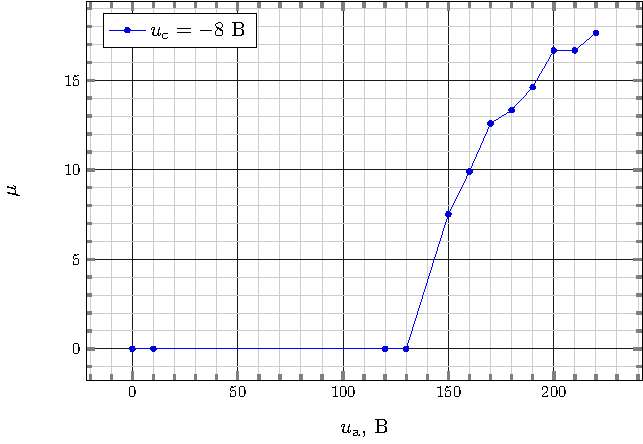
\includegraphics[]{fig/mu_from_ua.pdf}
	\vspace{-1em}
	\caption{Зависимость $\mu$ от напряжения на аноде}
	\label{fig:1}
\end{figure}
С увеличением напряжения на аноде, статический коэффициент усиления по напряжению увеличивается.
Данная зависимость объясняется аналогично предыдущей.

\addcontentsline{toc}{section}{Заключение}
\section*{Заключение}
В настоящей работе мы изучили принципы работы триода, сняли его анодную и анодно-сеточную характеристики, а так же зависимости статического коэффициента усиления по напряжению, внутреннего сопротивления и крутизны от напряжения на сетке и на аноде. 
\end{document}